\documentclass{article}
\usepackage[utf8]{inputenc}
\usepackage{graphicx}
\usepackage{pdfpages}
\usepackage[spanish]{babel}
\usepackage{pdfpages}
\usepackage{float}

\pagestyle{myheadings}
\markright{FIEE UNI \hfill Coeficientes de dilatación lineal \hfill}

% cabecera y pie
\usepackage{fancyhdr} % activamos el paquete
\pagestyle{fancy} % seleccionamos un estilo
\lhead{Informe de laboratorio FISICA II} % texto izquierda de la cabecera
\rhead{Coeficientes de dilatación lineal} % texto derecha de la cabecera
%\rhead{\thepage} % número de página a la derecha
\lfoot{FIEE-UNI} % texto izquierda del pie
%\cfoot{
\includegraphics[width=1cm]{uni}} % imagen centro del pie
%\rfoot{TEXTO} % texto derecha del pie
\cfoot{}
\rfoot{\thepage}
\renewcommand{\headrulewidth}{0.4pt} % grosor de la línea de la cabecera
\renewcommand{\footrulewidth}{0.4pt} % grosor de la línea del pie


\title{Informe de laboratorio de física 2: Coeficientes de dilatación lineal}
%\author{bseminarioa ,fddfsf,dfsdfsdf}
%\date{June 2017}

\begin{document}
%%%%%%%%%%%%%%%%%%%%%%%%%%%%%%INCLUYE PORTADA EN PDF%%%%%%%%%%%%%%%%%%%%%%&%%%%%%%%%%%%%%%%%%%%%%%%%%

\includepdf{PORTADA}
%%%%%%%%%%%%%%%%%%%$$$$$$$$$$$$$$$$$$$$$$$$$$$$$$$$$$$$$$$$$$$$$$$$$$$$$$$$$$$$$$$$$$$$$$$$$$$$$$$$$$$$$$$$$$$$


\tableofcontents
\newpage
%\maketitle
\section{Objetivos}
    Determinar el coeficiente de dilatación lineal de diferentes sustancias.
    % \LARGEAjusta el tamaño de las letras y la linea divisoria
    
 
%%%%%%%%%%%%%%%%%%%%%%%%%%%%%%%%%%%%%%%%%%%%%%%%%%%%%%%%%%%%%%%%%%%

\section{\\\\Marco teórico}
Las sustancias, contraen o incrementan su volumen al aumentar su temperatura.
En general la variación del tamaño de un cuerpo es en las tres dimensiones; sin embargo, debido a la geometría particular de cada cuerpo, en ciertos casos, sólo se considera el aumento de una dimensión o en dos dimensiones.


Cuando se considera sólo la dilatación en una dimensión se dice que se trata de una dilatación lineal, cuando es en dos dimensiones se le llama dilatación superficial y cuando es en tres se llama dilatación volumétrica.


Dicha dilatación depende, además de la sustancia de la que se trate, de las dimensiones iniciales y del incremento de temperatura.


Para el experimento en el laboratorio se estudiará el coeficiente de dilatación lineal.
Para el análisis cuantitativo de la dilatación del cuerpo es necesario definir un término conocido coeficiente de dilatación.

\subsection{Coeficiente de dilatación lineal ($\alpha$)}

Se define a este término como el aumento de longitud por aumento unitario de la temperatura. De esta manera, por ejemplo, si tenemos una varilla que aumenta 2mm después de haberla calentado de 20$^{\circ}$C a 21$^{\circ}$C, su coeficiente de dilatación lineal será:

    $$\alpha = 0.002(^{\circ}C)^{-1}$$
\hbox{ddfdfdfdf}
$$\Delta = \alpha L_{0} \Delta T$$
$$\Delta L = R_{A} \theta$$

$$\alpha = 2(r_{A}.\theta_{B})$$
$$L_{f} = L_{0}(1 + \alpha\Delta T)$$
$$L_{f} = L_{0} + L_{0} \alpha\Delta T$$
$$L_{f} - L_{0} =  \alpha L_{0} \Delta T)$$
$$\Delta L = \alpha L_{0} \Delta T$$
$$\alpha = \frac{\Delta L}{L_{0} \Delta T}$$


Análogamente puede definirse el coeficiente de dilatación superficial y el coeficiente de dilatación volumétrica.
\newpage
%%%%%%%%%%%%%%%%%%%%%%%%%%%%%%%%%%%%%%%%%%%%%%%%%%%%%%%%%%%%%%%%%%%%%%%%%%%%
\section{Montaje experimental}

\subsection{Equipo y materiales}
\begin{enumerate}
    \item Una fuente de vapor
	\item Un aparato de dilatación térmica lineal %(El aparato que mide la variación de longitud es un disco de cartón atravesado por una aguja)sobre la q
	\itposa la varillem.
	ue re Unaa  regla de un metro, graduada en milímetros
	\item Una regla de un metro, graduada en milímetros
	\item Tres tubos: (cobre, aluminio y vidrio)
	\item Un transportador
	\item Un Vernier
\end{enumerate}
\begin{figure}[H]
    \centering
    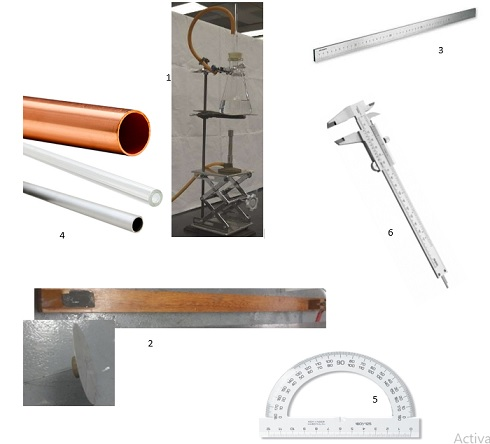
\includegraphics{materiales}
    \caption{Las imágenes son referenciales}
    \label{fig:my_label}
\end{figure}
    

\subsection{Procedimiento experimental\\\\}
\begin{enumerate}
    \item Se debe disponer el equipo teniendo en cuenta que la varilla debe tener un punto fijo sujetado por una pinza donde a su vez se conectara el tubo por donde saldrá el vapor, y por el otro lado estará sujetando una aguja conectada a un indicador, que girará cuando el tubo aumente su longitud.\\\\
    
    \item El valor del aumento de la temperatura puede obtenerse teniendo en cuenta que la temperatura inicial es la del ambiente y la temperatura final sería aproximadamente 100$^{\circ}$C debido a que es la temperatura del vapor de agua que pasará por el tubo.\\\\

    \item Luego el ángulo que gira la aguja se puede medir fácilmente con ayuda del indicador y a partir de este ángulo calcular la dilatación lineal.\\\\

    \item Para este cálculo debe tenerse en cuenta que el eje de la aguja se traslada mientras ella gira así que la dilatación no será el producto del radio por el ángulo girado sino el doble de este valor.\\

\end{enumerate}
\newpage
%%%%%%%%%%%%%%%%%%%%%%%%%%%%%%%%%%%%%%%%%%%%%%%%%%%%%%%%%%%%%%%%%%%%%%%%%%%%%
\section{Cálculos y análisis de datos}
\subsection{Datos recolectados}

\begin{table}[H]
    \centering
        \begin{tabular}{|c|c|c|}
        \hline
        \textfb{Material} & \textfb{Longitud inicial} & \textfb{Ángulo}  \\
        \hline
        Cobre & 55,6 & 35$^{\circ}$ \\
        \hline
        Vidrio & 55,6 & 155$^{\circ}$\\
        \hline
        Aluminio & 55,6 & 6$^{\circ}$\\
        \hline
    \end{tabular}
    %\caption{Caption}
    \label{tab:my_label}
\end{table}

\begin{itemize}
    \item Diámetro del disco      5,7cm
    \item Diámetro de la aguja  0,55mm
\end{itemize}

\subsection{Cálculos}
\begin{table}[H]
    \centering
    \begin{tabular}{|c|c|c|c|}
    \hline \hline
    \textfb{MATERIAL} & \textfb{LONGITUD INICIAL}	& \textfb{ANGULO}	& \textfb{ÁNGULO (radianes)\\}
    \hline \hline
     COBRE &	556 mm &	35$^{circ}$ &	0.611\\
    \hline
    ALUMINIO &	556 mm &	155$^{circ}$ &	2.71\\
    \hline
    VIDRIO &	556 mm	& 6$^{circ}$ &	0.105\\
    \hline 
    \end{tabular}
    \caption{Caption}
    \label{tab:my_label}
\end{table}
\begin{itemize}
    \item Radio de la aguja :  0.275 mm
\end{itemize}

\\Para el tubo de cobre 


    $$\Delta L = 2 (R_{A}.\theta)$$
    $$\Delta L = 0.33605 mm$$
    $$\Delta T = 100 ^{\circ}C - 19 ^{\circ}= 81 ^{\circ}$$
    
    $$\alpha_{cobre} = \frac{\Delta L}{L_{0}.\Delta T}$$
    $$\alpha_{cobre} = 7,5 . 10^{-6}^{\circ}  C^{-1}$$
    Error relativo para el tubo de cobre\\

$$Valor teórico = 1,7.10^{-5}  ^{\circ}C^{-1}$$
$$Valor experimental = 7,5.10^{-6}  ^{\circ}C^{-1}$$


$$Error relativo = \frac{\abs{1,7.10^{-5} - 7,5.10^{-6}}}{1,7.10^{-5}} = 55,88 \% $$

%%%%%%%%%%%%%%%%%%%%%%%%%%%%

Para el tubo de aluminio:
    $$\Delta L = 2 (R_{A}.\theta)$$
    $$\Delta L = 1.4905 mm$$
    $$\Delta T = 100 ^{\circ}C - 19 ^{\circ}= 81 ^{\circ}$$
    
    $$\alpha_{aluminio} = \frac{\Delta L}{L_{0}.\Delta T}$$
    $$\alpha_{aluminio} = 3,31 . 10^{-5}^{\circ}  C^{-1}$$

\\Error relativo para el tubo de aluminio:\\
$$Valor teórico = 2,4.10^{-5}  ^{\circ}C^{-1}$$
$$Valor experimental = 3,31.10^{-5}  ^{\circ}C^{-1}$$

$$Error relativo = \frac{\abs{2,4.10^{-5} - 3,31.10^{-5}  }}{2,4.10^{-5}} = 37,92 \% $$


%%%%%%%%%%%%%%%%%%%%%%%
\\Para el tubo de vidrio:\\


    $$\Delta L = 2 (R_{A}.\theta)$$
    $$\Delta L = 0.05775 mm$$
    $$\Delta T = 100 ^{\circ}C - 19 ^{\circ}= 81 ^{\circ}$$
    
    $$\alpha_{vidrio} = \frac{\Delta L}{L_{0}.\Delta T}$$
    $$\alpha_{vidrio} = 1,28 . 10^{-6}^{\circ}  C^{-1}$$

\\Error relativo para el tubo de vidrio:\\

$$Valor teórico = 3,2.10^{-6}  ^{\circ}C^{-1}$$
$$Valor experimental = 1,28.10^{-6}  ^{\circ}C^{-1}$$

$$Error relativo = \frac{\abs{3,2.10^{-6} - 1,28.10^{-6}  }}{3,2.10^{-6}} = 60 \% $$

\newpage



%%%%%%%%%%%%%%%%%%%%%%%%%%%%%%%%%%%%%%%%%%%%%%%%%%%%%%%%%%%%
\section{Conclusiones y observaciones}
\subsection{Conclusiones}

\subsection{Observaciones}

\newpage

%%%%%%%%%%%%%%%%%%%%%%%%%%%%%%%%%%%%%%%%%%%%%%%%%%%%%%%%%%%%%%%%%%%%
\begin{thebibliography}

\end{thebibliography}
\end{document}
